\documentclass[tikz,border=2pt]{standalone}
\usepackage{amsmath,amssymb}
\usepackage{tikz}
\usetikzlibrary{arrows.meta}

\begin{document}
% The incumbent is the best integer-feasible solution found so far; it only improves over
% time and its value L is the yardstick for pruning.
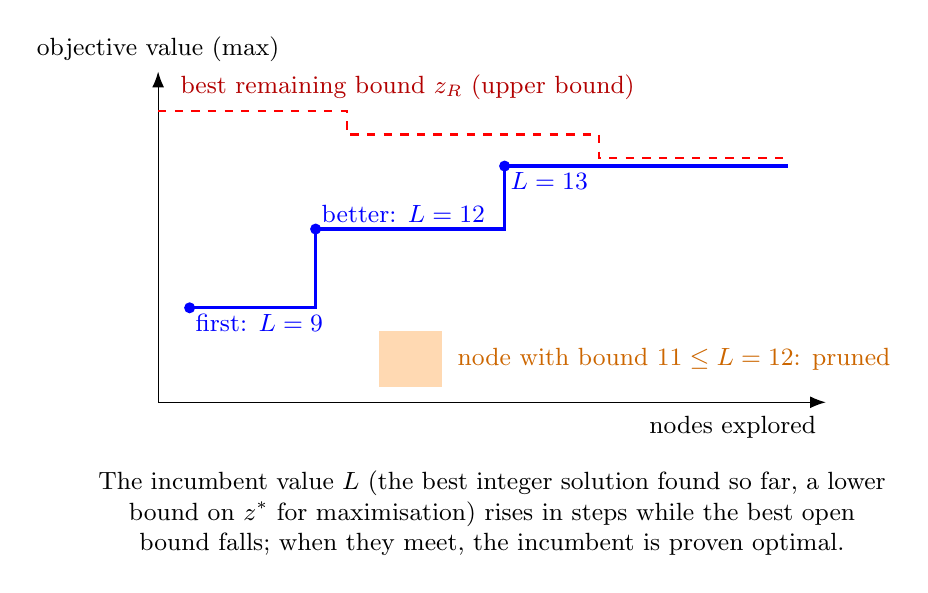
\begin{tikzpicture}[x=0.8cm, every node/.style={font=\small}, >={Latex[length=2mm]}]
	\draw[->] (0,0) -- (10.6,0);
	\node[anchor=north east] at (10.6,-0.05) {nodes explored};
	\draw[->] (0,0) -- (0,4.2) node[above] {objective value (max)};
	\draw[blue, very thick] (0.5,1.2) -- (2.5,1.2) -- (2.5,2.2) -- (5.5,2.2) -- (5.5,3.0) -- (10,3.0);
	\fill[blue] (0.5,1.2) circle (2pt) node[below right, inner sep=2pt] {first: $L=9$};
	\fill[blue] (2.5,2.2) circle (2pt) node[above right, inner sep=2pt] {better: $L=12$};
	\fill[blue] (5.5,3.0) circle (2pt) node[below right, inner sep=2pt] {$L=13$};
	\draw[red, dashed, thick] (0,3.7) -- (3,3.7) -- (3,3.4) -- (7,3.4) -- (7,3.1) -- (10,3.1);
	\node[red!70!black, anchor=south west] at (0.2,3.72) {best remaining bound $z_R$ (upper bound)};
	\fill[orange!30] (3.5,0.2) rectangle (4.5,0.9);
	\node[orange!80!black, anchor=west] at (4.6,0.55) {node with bound $11\le L=12$: pruned};
	\node[anchor=north, align=flush center, text width=10cm] at (5.3,-0.75) {The incumbent value $L$ (the best integer solution found so far, a lower bound on $z^\ast$ for maximisation) rises in steps while the best open bound falls; when they meet, the incumbent is proven optimal.};
\end{tikzpicture}
\end{document}
